%
% $Id: appa--code
%
%   *******************************************************************
%   * SEE THE MAIN FILE "AllegThesis.tex" FOR MORE INFORMATION.       *
%   *******************************************************************

\chapter{Data Visualizations}\label{appa:data}
This Appendix contains the full set of data visualizations.  The graphs are presented in grids, with with each grid containing the playouts between two different agents; each grid contains all board sizes and time allowances for these agents.  They are organized with board size increasing left to right, and the time allowance increasing from top to bottom.  For example, 5x5 Go games with a 500ms time allowance are in the top-left corner of each grid, while 11x11 Go games with an 8000ms time allowance are in the bottom right.

For a demonstration of how to read a graph containing the score information for a board configuration of Go, consider Figure\ref{fig:apex}.  In addition to giving the board size and time allowance of the game, the graph is titled in order of player; that is, it is formatted as `Player one' vs `Player two'.  This distinction is important to properly understand the score.  The x-axis is how many moves have been made in a game, and the y-axis notates the score of the game at that point.  Each colored line on the graph represents a single, distinct playout of the game.  A positive score is good for Player one, and a negative score is good for Player 2.  The grey smooth curve represents the average score at each move across all games of that type.

\begin{figure}[h]
  \centering
  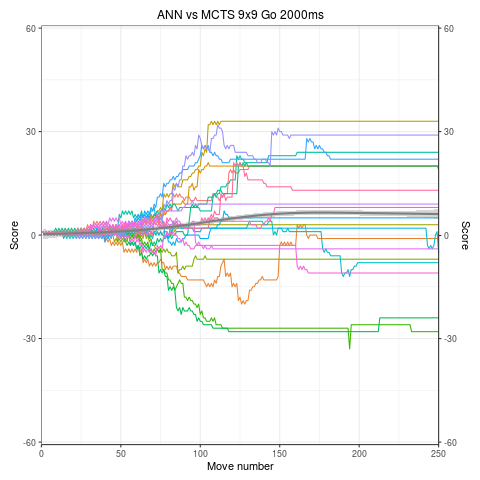
\includegraphics[scale=0.6]{images/Visualizations/ANNvsMCTS/2000ms9x9.png}
  \caption{Go Score Sample Graph}
  \label{fig:apex}
\end{figure}

\begin{figure}
\centering
\begin{tabular}{cccc}
\hspace{-0.5cm}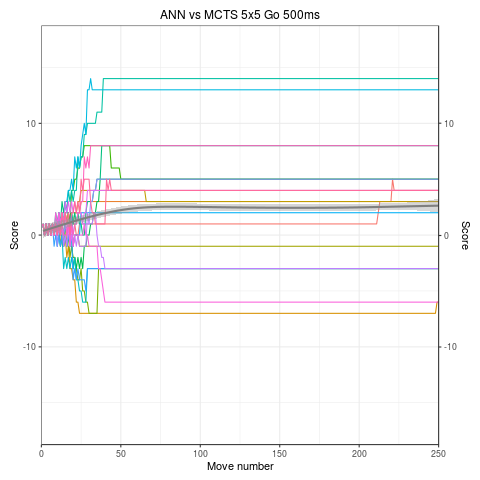
\includegraphics[width = 1.55in]{images/Visualizations/ANNvsMCTS/500ms5x5.png} &
\hspace{-0.5cm}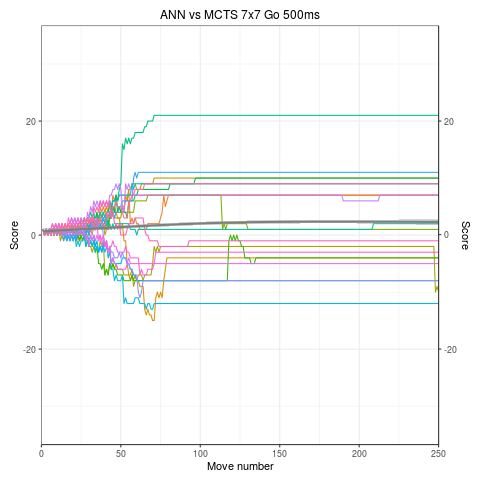
\includegraphics[width = 1.55in]{images/Visualizations/ANNvsMCTS/500ms7x7.png} &
\hspace{-0.5cm}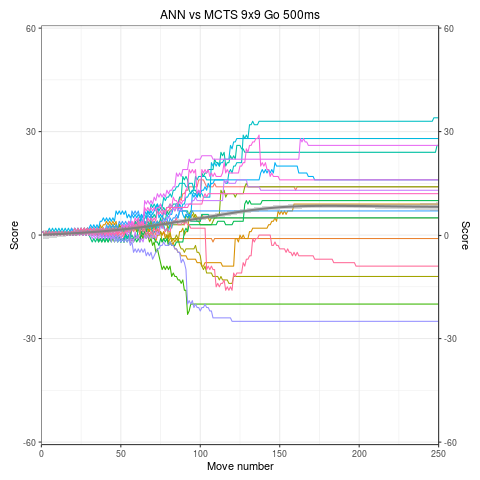
\includegraphics[width = 1.55in]{images/Visualizations/ANNvsMCTS/500ms9x9.png} &
\hspace{-0.5cm}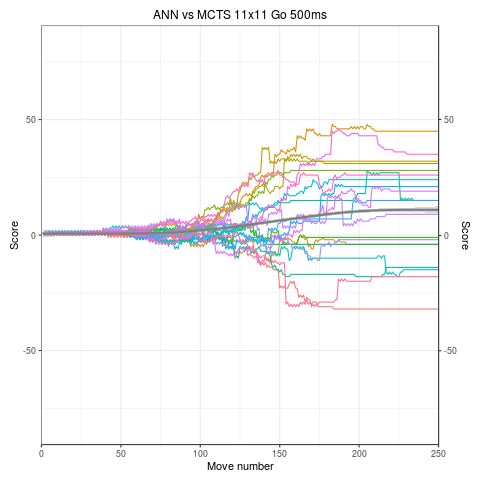
\includegraphics[width = 1.55in]{images/Visualizations/ANNvsMCTS/500ms11x11.png} \\

\hspace{-0.5cm}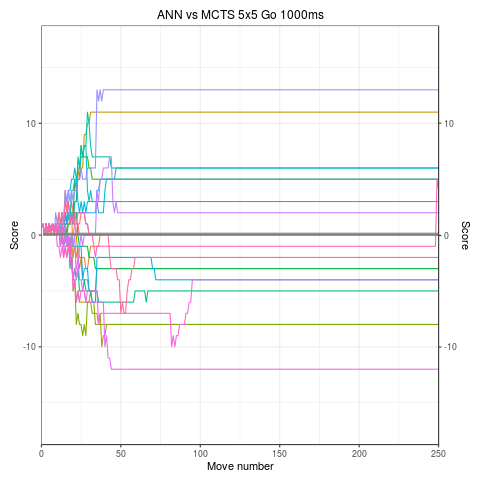
\includegraphics[width = 1.55in]{images/Visualizations/ANNvsMCTS/1000ms5x5.png} &
\hspace{-0.5cm}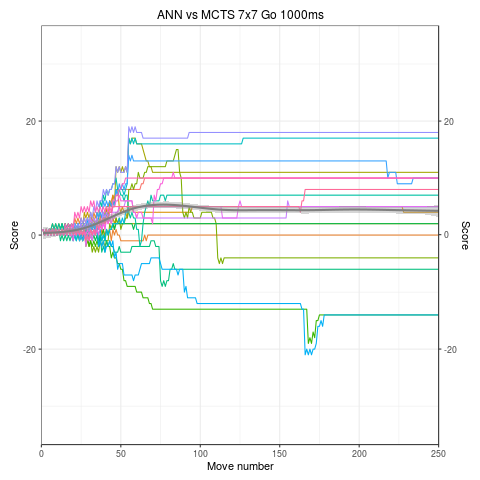
\includegraphics[width = 1.55in]{images/Visualizations/ANNvsMCTS/1000ms7x7.png} &
\hspace{-0.5cm}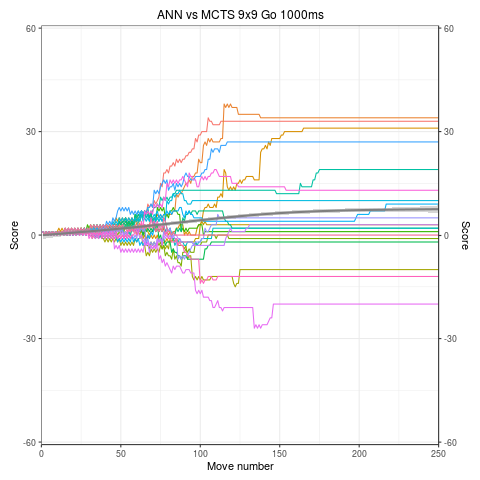
\includegraphics[width = 1.55in]{images/Visualizations/ANNvsMCTS/1000ms9x9.png} &
\hspace{-0.5cm}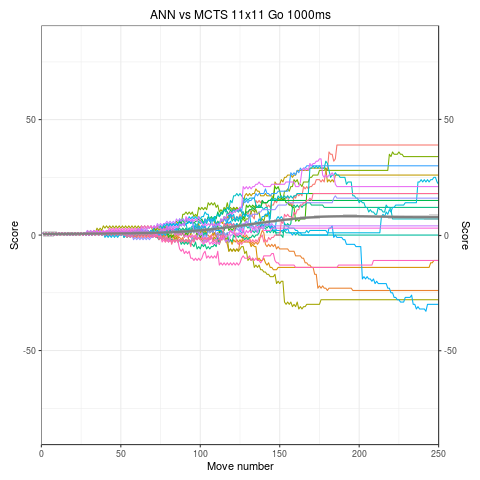
\includegraphics[width = 1.55in]{images/Visualizations/ANNvsMCTS/1000ms11x11.png} \\

\hspace{-0.5cm}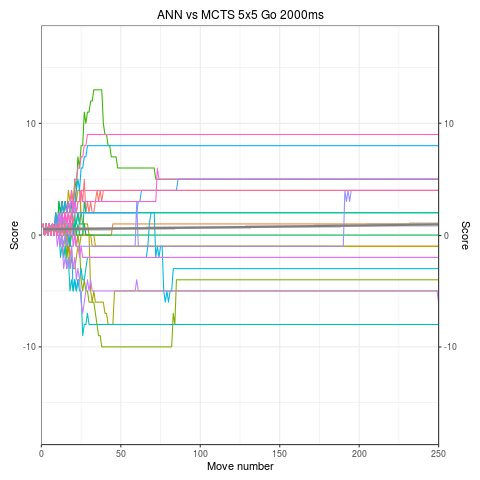
\includegraphics[width = 1.55in]{images/Visualizations/ANNvsMCTS/2000ms5x5.png} &
\hspace{-0.5cm}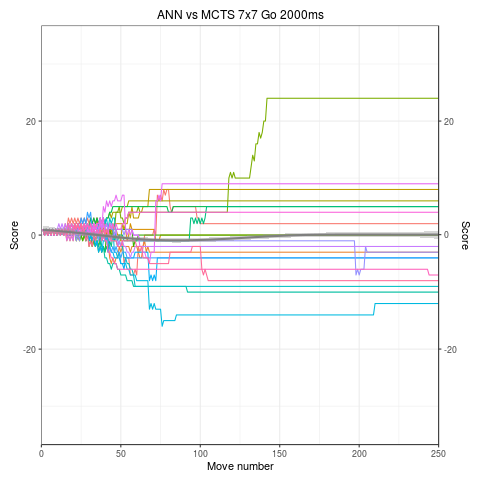
\includegraphics[width = 1.55in]{images/Visualizations/ANNvsMCTS/2000ms7x7.png} &
\hspace{-0.5cm}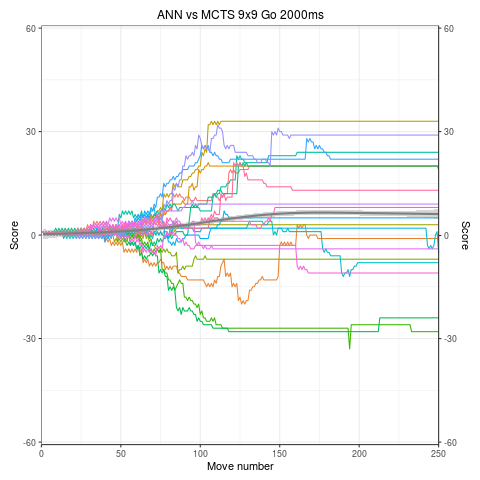
\includegraphics[width = 1.55in]{images/Visualizations/ANNvsMCTS/2000ms9x9.png} &
\hspace{-0.5cm}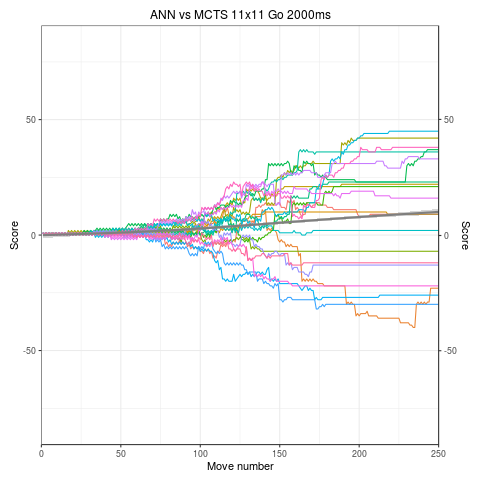
\includegraphics[width = 1.55in]{images/Visualizations/ANNvsMCTS/2000ms11x11.png} \\

\hspace{-0.5cm}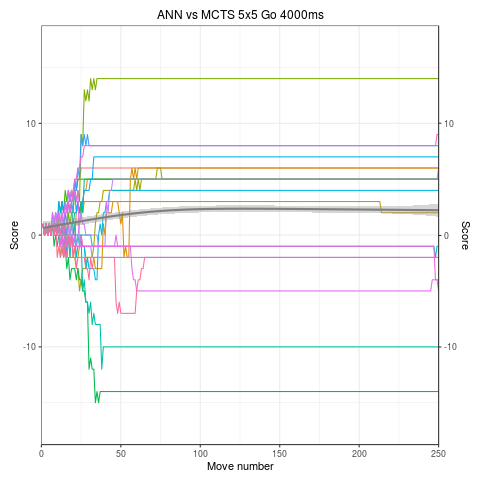
\includegraphics[width = 1.55in]{images/Visualizations/ANNvsMCTS/4000ms5x5.png} &
\hspace{-0.5cm}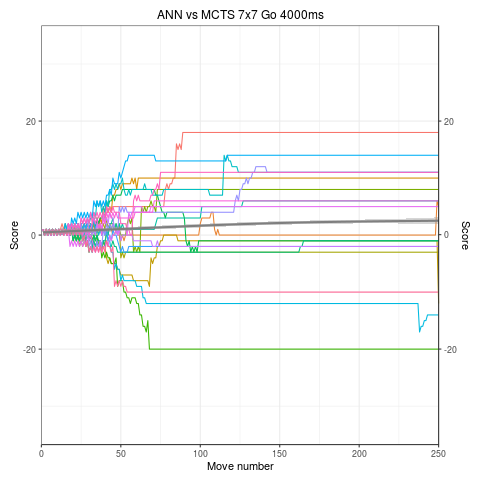
\includegraphics[width = 1.55in]{images/Visualizations/ANNvsMCTS/4000ms7x7.png} &
\hspace{-0.5cm}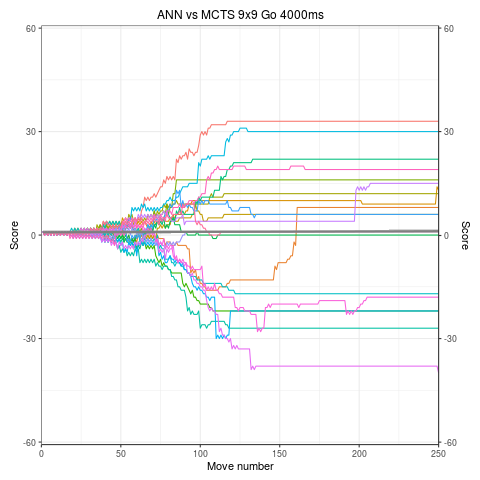
\includegraphics[width = 1.55in]{images/Visualizations/ANNvsMCTS/4000ms9x9.png} &
\hspace{-0.5cm}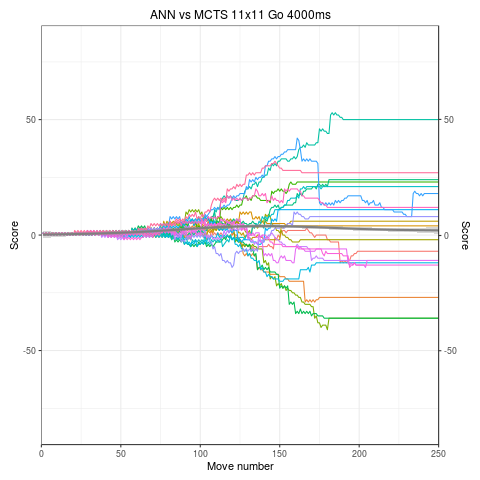
\includegraphics[width = 1.55in]{images/Visualizations/ANNvsMCTS/4000ms11x11.png} \\

\hspace{-0.5cm}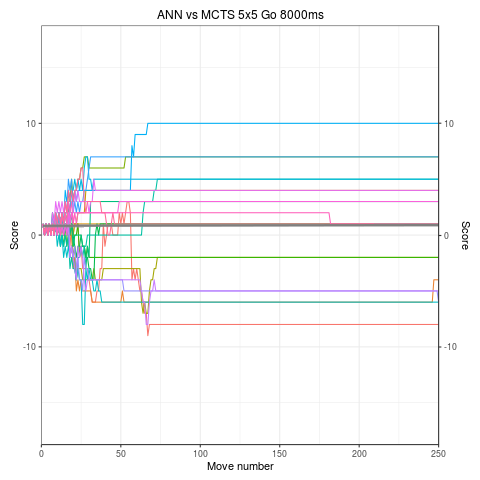
\includegraphics[width = 1.55in]{images/Visualizations/ANNvsMCTS/8000ms5x5.png} &
\hspace{-0.5cm}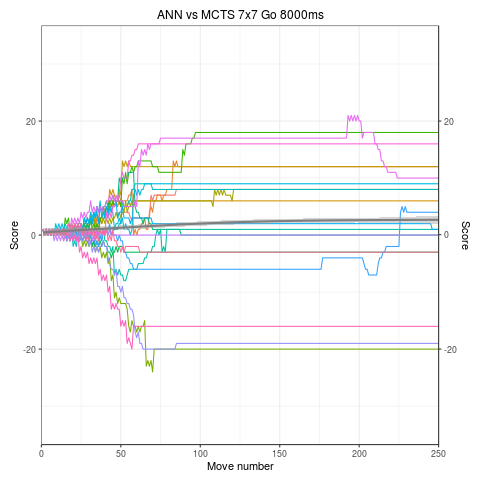
\includegraphics[width = 1.55in]{images/Visualizations/ANNvsMCTS/8000ms7x7.png} &
\hspace{-0.5cm}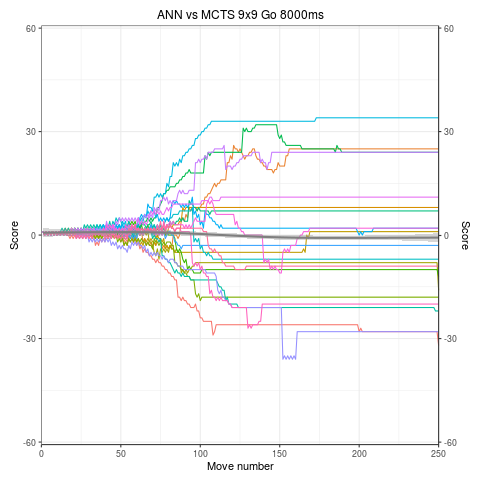
\includegraphics[width = 1.55in]{images/Visualizations/ANNvsMCTS/8000ms9x9.png} &
\hspace{-0.5cm}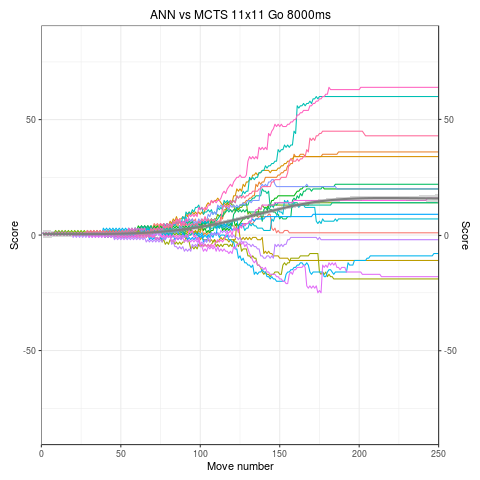
\includegraphics[width = 1.55in]{images/Visualizations/ANNvsMCTS/8000ms11x11.png} \\
\end{tabular}
\caption{\texttt{ANNAgent} vs \texttt{MCTSAgent} Go scores by board size and time allowance}
\label{app:annmctsscore}
\end{figure}

\begin{figure}
\centering
\begin{tabular}{cccc}
\hspace{-0.5cm}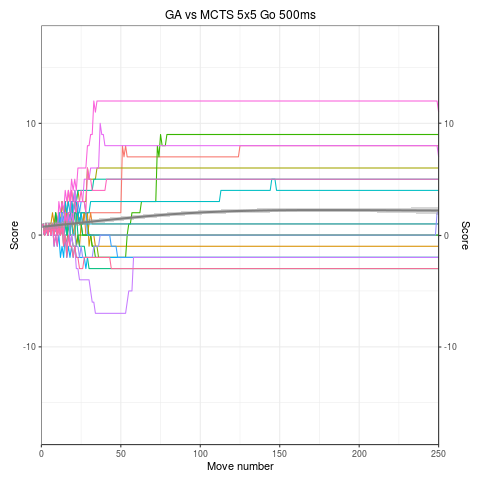
\includegraphics[width = 1.55in]{images/Visualizations/GAvsMCTS/500ms5x5.png} &
\hspace{-0.5cm}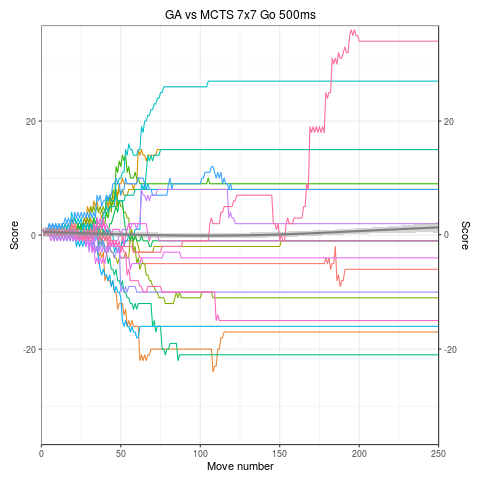
\includegraphics[width = 1.55in]{images/Visualizations/GAvsMCTS/500ms7x7.png} &
\hspace{-0.5cm}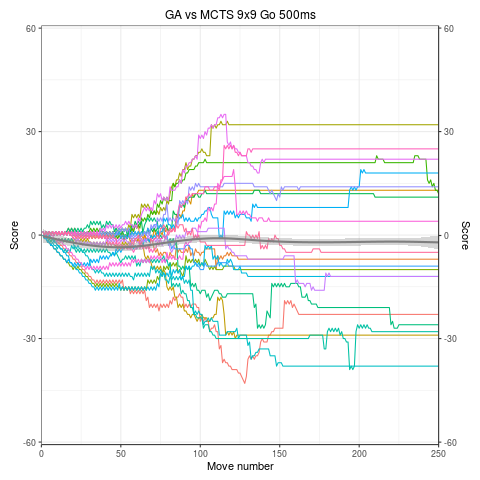
\includegraphics[width = 1.55in]{images/Visualizations/GAvsMCTS/500ms9x9.png} &
\hspace{-0.5cm}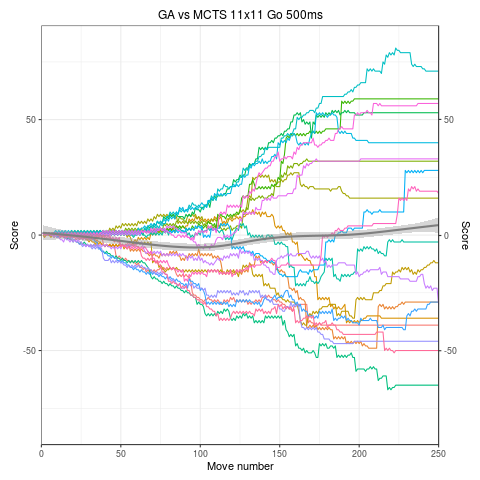
\includegraphics[width = 1.55in]{images/Visualizations/GAvsMCTS/500ms11x11.png} \\

\hspace{-0.5cm}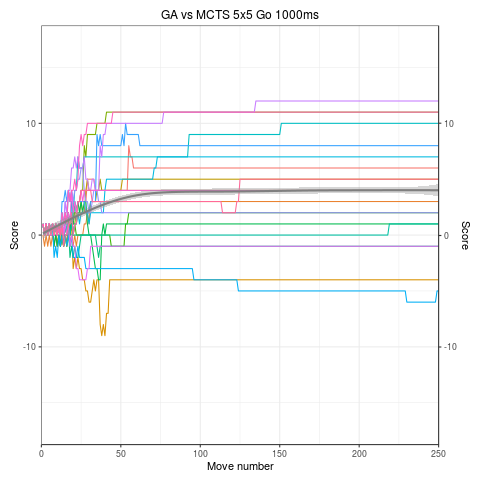
\includegraphics[width = 1.55in]{images/Visualizations/GAvsMCTS/1000ms5x5.png} &
\hspace{-0.5cm}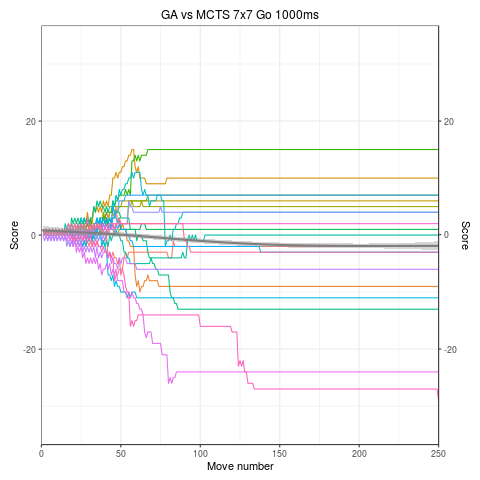
\includegraphics[width = 1.55in]{images/Visualizations/GAvsMCTS/1000ms7x7.png} &
\hspace{-0.5cm}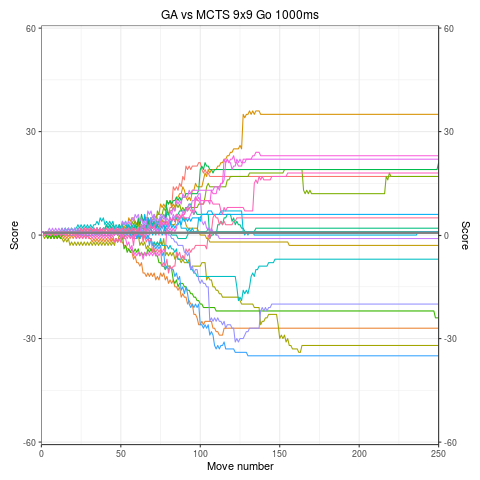
\includegraphics[width = 1.55in]{images/Visualizations/GAvsMCTS/1000ms9x9.png} &
\hspace{-0.5cm}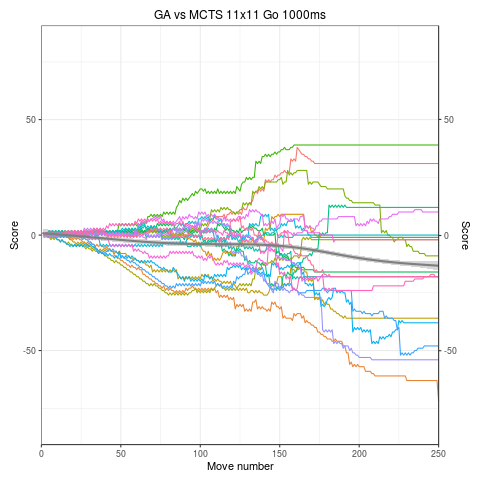
\includegraphics[width = 1.55in]{images/Visualizations/GAvsMCTS/1000ms11x11.png} \\

\hspace{-0.5cm}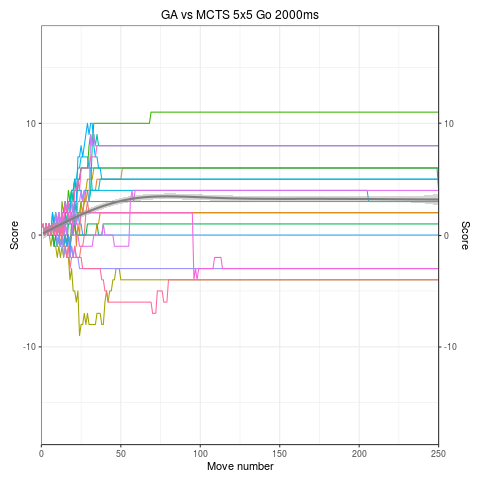
\includegraphics[width = 1.55in]{images/Visualizations/GAvsMCTS/2000ms5x5.png} &
\hspace{-0.5cm}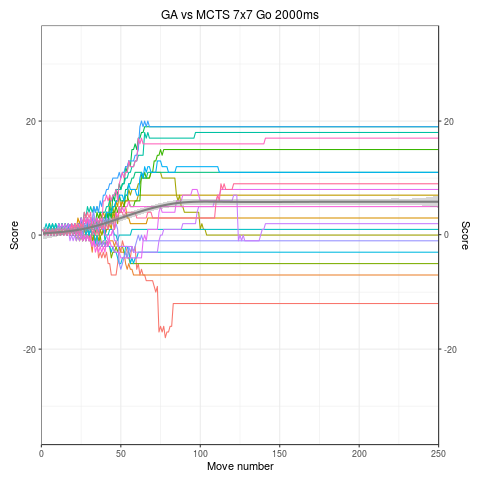
\includegraphics[width = 1.55in]{images/Visualizations/GAvsMCTS/2000ms7x7.png} &
\hspace{-0.5cm}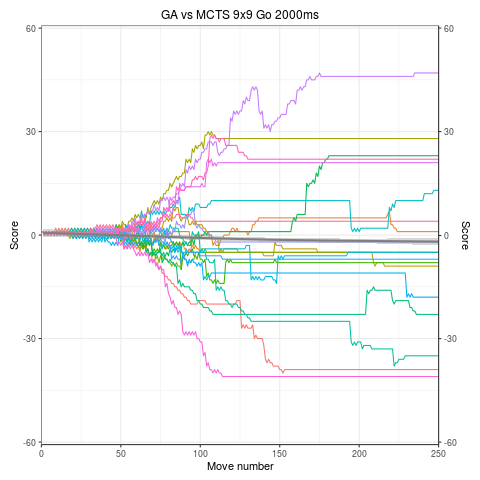
\includegraphics[width = 1.55in]{images/Visualizations/GAvsMCTS/2000ms9x9.png} &
\hspace{-0.5cm}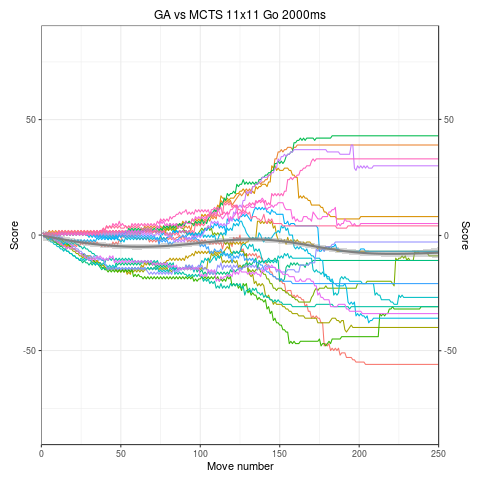
\includegraphics[width = 1.55in]{images/Visualizations/GAvsMCTS/2000ms11x11.png} \\

\hspace{-0.5cm}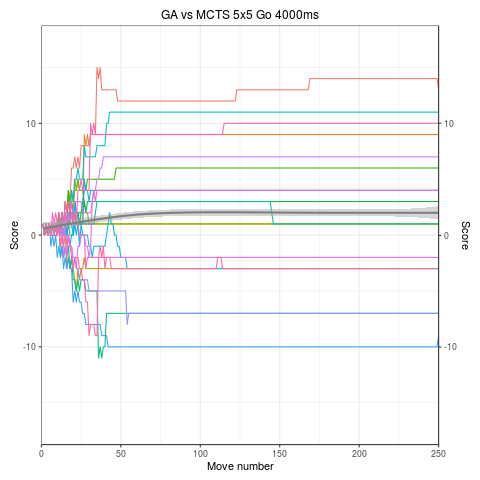
\includegraphics[width = 1.55in]{images/Visualizations/GAvsMCTS/4000ms5x5.png} &
\hspace{-0.5cm}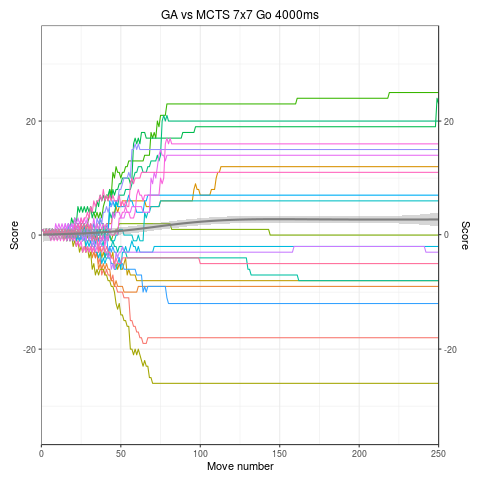
\includegraphics[width = 1.55in]{images/Visualizations/GAvsMCTS/4000ms7x7.png} &
\hspace{-0.5cm}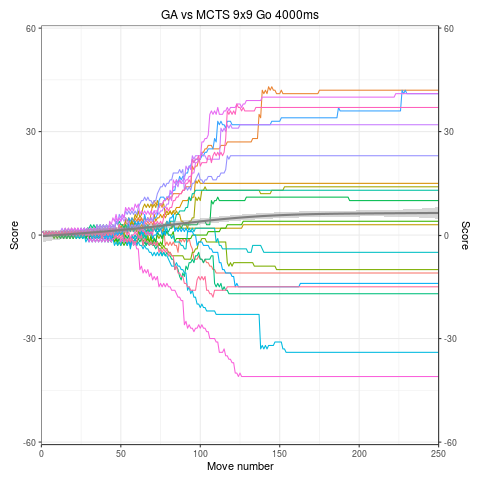
\includegraphics[width = 1.55in]{images/Visualizations/GAvsMCTS/4000ms9x9.png} &
\hspace{-0.5cm}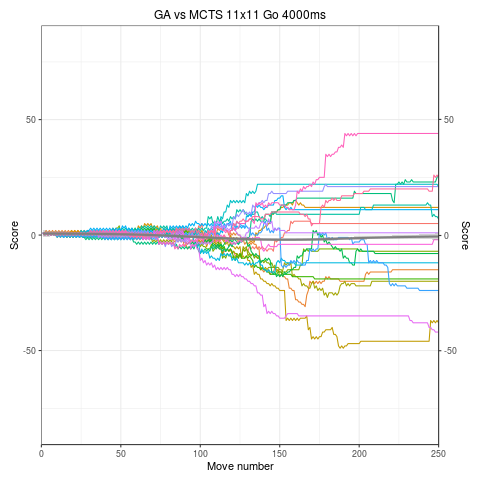
\includegraphics[width = 1.55in]{images/Visualizations/GAvsMCTS/4000ms11x11.png} \\

\hspace{-0.5cm}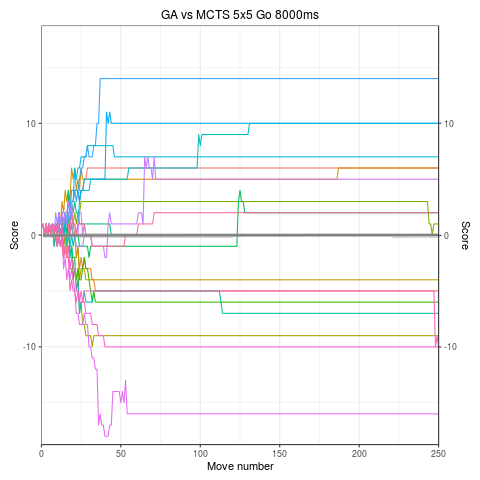
\includegraphics[width = 1.55in]{images/Visualizations/GAvsMCTS/8000ms5x5.png} &
\hspace{-0.5cm}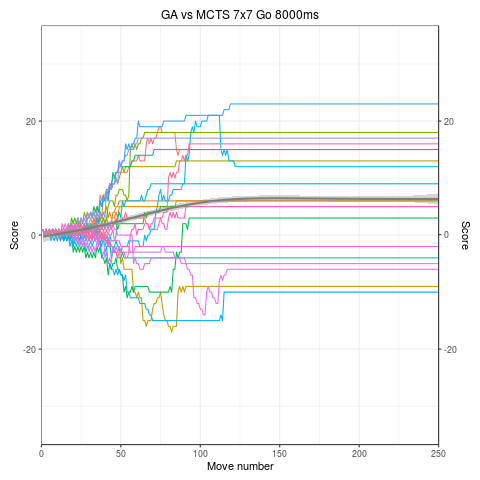
\includegraphics[width = 1.55in]{images/Visualizations/GAvsMCTS/8000ms7x7.png} &
\hspace{-0.5cm}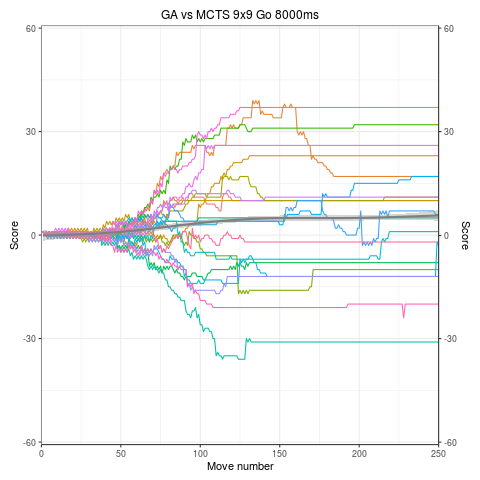
\includegraphics[width = 1.55in]{images/Visualizations/GAvsMCTS/8000ms9x9.png} &
\hspace{-0.5cm}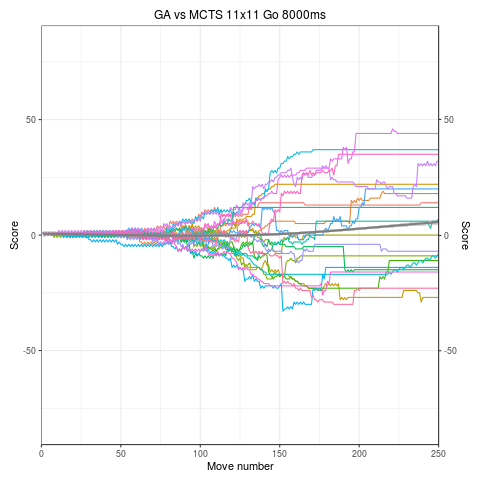
\includegraphics[width = 1.55in]{images/Visualizations/GAvsMCTS/8000ms11x11.png} \\
\end{tabular}
\caption{\texttt{GAAgent} vs \texttt{MCTSAgent} Go scores by board size and time allowance}
\label{app:gamctsscore}
\end{figure}

\begin{figure}
\centering
\begin{tabular}{cccc}
\hspace{-0.5cm}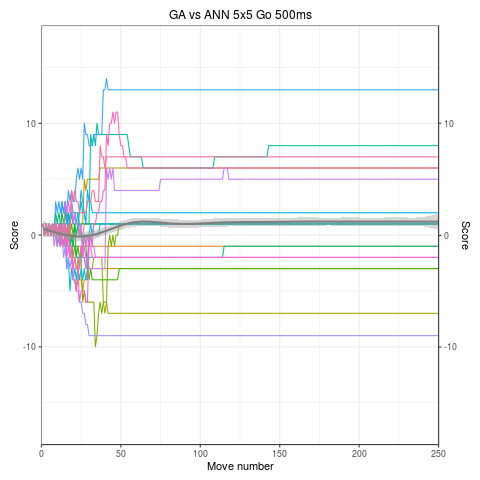
\includegraphics[width = 1.55in]{images/Visualizations/GAvsANN/500ms5x5.png} &
\hspace{-0.5cm}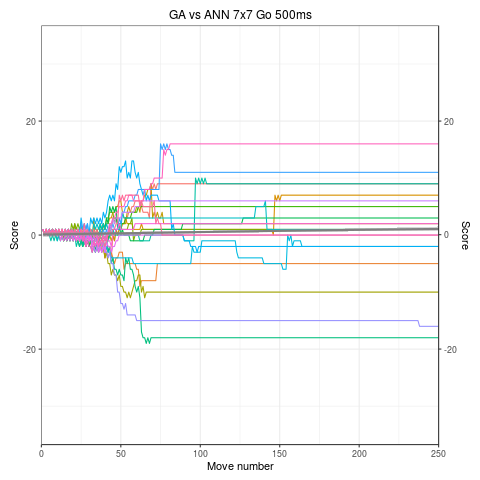
\includegraphics[width = 1.55in]{images/Visualizations/GAvsANN/500ms7x7.png} &
\hspace{-0.5cm}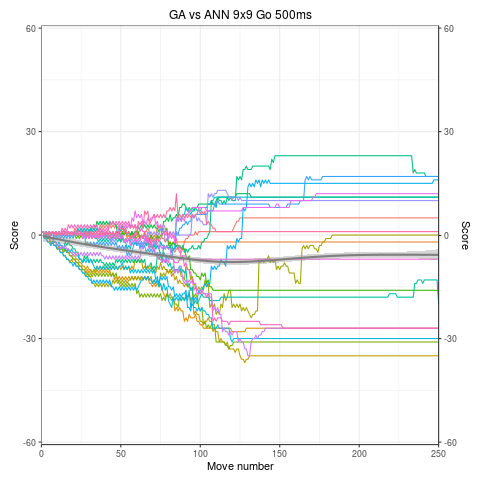
\includegraphics[width = 1.55in]{images/Visualizations/GAvsANN/500ms9x9.png} &
\hspace{-0.5cm}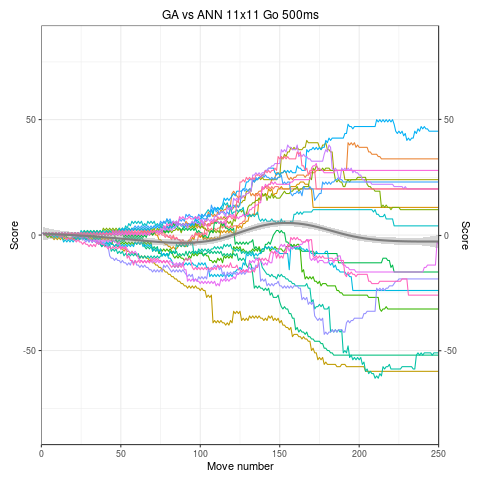
\includegraphics[width = 1.55in]{images/Visualizations/GAvsANN/500ms11x11.png} \\

\hspace{-0.5cm}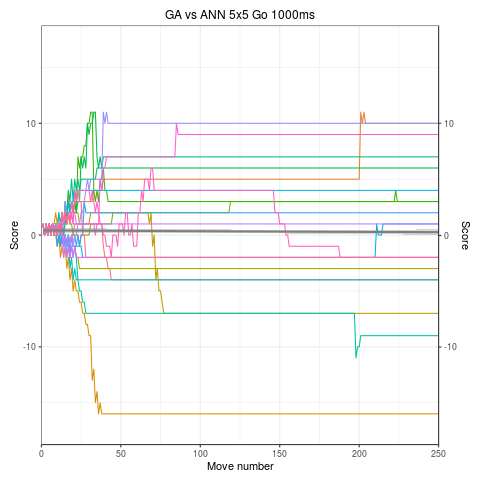
\includegraphics[width = 1.55in]{images/Visualizations/GAvsANN/1000ms5x5.png} &
\hspace{-0.5cm}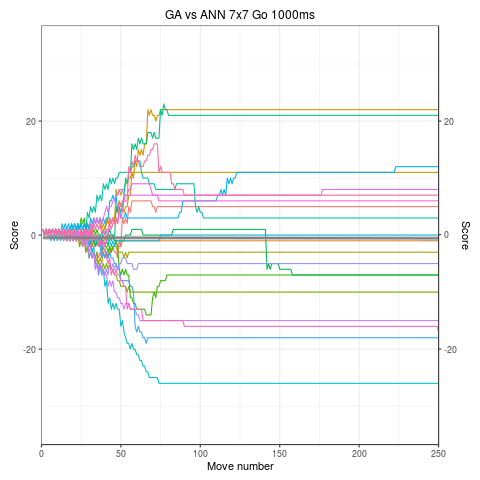
\includegraphics[width = 1.55in]{images/Visualizations/GAvsANN/1000ms7x7.png} &
\hspace{-0.5cm}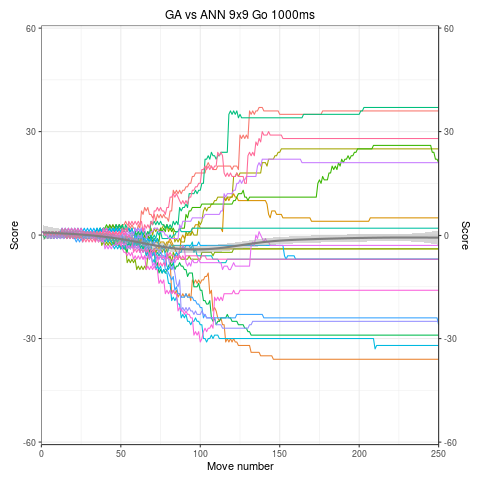
\includegraphics[width = 1.55in]{images/Visualizations/GAvsANN/1000ms9x9.png} &
\hspace{-0.5cm}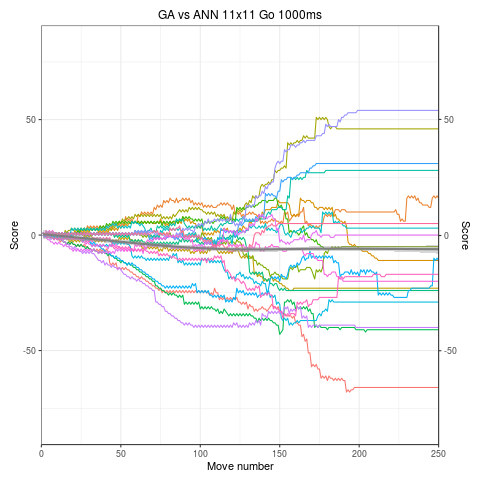
\includegraphics[width = 1.55in]{images/Visualizations/GAvsANN/1000ms11x11.png} \\

\hspace{-0.5cm}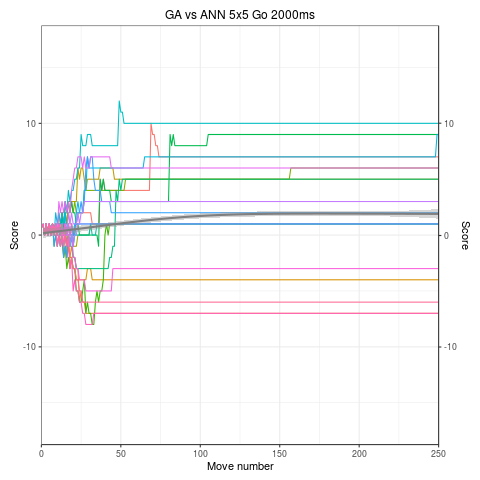
\includegraphics[width = 1.55in]{images/Visualizations/GAvsANN/2000ms5x5.png} &
\hspace{-0.5cm}\includegraphics[width = 1.55in]{images/Visualizations/GAvsANN/2000ms7x7.png} &
\hspace{-0.5cm}\includegraphics[width = 1.55in]{images/Visualizations/GAvsANN/2000ms9x9.png} &
\hspace{-0.5cm}\includegraphics[width = 1.55in]{images/Visualizations/GAvsANN/2000ms11x11.png} \\

\hspace{-0.5cm}\includegraphics[width = 1.55in]{images/Visualizations/GAvsANN/4000ms5x5.png} &
\hspace{-0.5cm}\includegraphics[width = 1.55in]{images/Visualizations/GAvsANN/4000ms7x7.png} &
\hspace{-0.5cm}\includegraphics[width = 1.55in]{images/Visualizations/GAvsANN/4000ms9x9.png} &
\hspace{-0.5cm}\includegraphics[width = 1.55in]{images/Visualizations/GAvsANN/4000ms11x11.png} \\

\hspace{-0.5cm}\includegraphics[width = 1.55in]{images/Visualizations/GAvsANN/8000ms5x5.png} &
\hspace{-0.5cm}\includegraphics[width = 1.55in]{images/Visualizations/GAvsANN/8000ms7x7.png} &
\hspace{-0.5cm}\includegraphics[width = 1.55in]{images/Visualizations/GAvsANN/8000ms9x9.png} &
\hspace{-0.5cm}\includegraphics[width = 1.55in]{images/Visualizations/GAvsANN/8000ms11x11.png} \\
\end{tabular}
\caption{\texttt{GAAgent} vs \texttt{ANNAgent} Go scores by board size and time allowance}
\label{app:gaannscore}
\end{figure}

\begin{figure}
\centering
\begin{tabular}{cccc}
\hspace{-0.5cm}\includegraphics[width = 1.55in]{images/Visualizations/MCTSvsRANDOM/500ms5x5.png} &
\hspace{-0.5cm}\includegraphics[width = 1.55in]{images/Visualizations/MCTSvsRANDOM/500ms7x7.png} &
\hspace{-0.5cm}\includegraphics[width = 1.55in]{images/Visualizations/MCTSvsRANDOM/500ms9x9.png} &
\hspace{-0.5cm}\includegraphics[width = 1.55in]{images/Visualizations/MCTSvsRANDOM/500ms11x11.png} \\

\hspace{-0.5cm}\includegraphics[width = 1.55in]{images/Visualizations/MCTSvsRANDOM/1000ms5x5.png} &
\hspace{-0.5cm}\includegraphics[width = 1.55in]{images/Visualizations/MCTSvsRANDOM/1000ms7x7.png} &
\hspace{-0.5cm}\includegraphics[width = 1.55in]{images/Visualizations/MCTSvsRANDOM/1000ms9x9.png} &
\hspace{-0.5cm}\includegraphics[width = 1.55in]{images/Visualizations/MCTSvsRANDOM/1000ms11x11.png} \\

\hspace{-0.5cm}\includegraphics[width = 1.55in]{images/Visualizations/MCTSvsRANDOM/2000ms5x5.png} &
\hspace{-0.5cm}\includegraphics[width = 1.55in]{images/Visualizations/MCTSvsRANDOM/2000ms7x7.png} &
\hspace{-0.5cm}\includegraphics[width = 1.55in]{images/Visualizations/MCTSvsRANDOM/2000ms9x9.png} &
\hspace{-0.5cm}\includegraphics[width = 1.55in]{images/Visualizations/MCTSvsRANDOM/2000ms11x11.png} \\

\hspace{-0.5cm}\includegraphics[width = 1.55in]{images/Visualizations/MCTSvsRANDOM/4000ms5x5.png} &
\hspace{-0.5cm}\includegraphics[width = 1.55in]{images/Visualizations/MCTSvsRANDOM/4000ms7x7.png} &
\hspace{-0.5cm}\includegraphics[width = 1.55in]{images/Visualizations/MCTSvsRANDOM/4000ms9x9.png} &
\hspace{-0.5cm}\includegraphics[width = 1.55in]{images/Visualizations/MCTSvsRANDOM/4000ms11x11.png} \\

\hspace{-0.5cm}\includegraphics[width = 1.55in]{images/Visualizations/MCTSvsRANDOM/8000ms5x5.png} &
\hspace{-0.5cm}\includegraphics[width = 1.55in]{images/Visualizations/MCTSvsRANDOM/8000ms7x7.png} &
\hspace{-0.5cm}\includegraphics[width = 1.55in]{images/Visualizations/MCTSvsRANDOM/8000ms9x9.png} &
\hspace{-0.5cm}\includegraphics[width = 1.55in]{images/Visualizations/MCTSvsRANDOM/8000ms11x11.png} \\
\end{tabular}
\caption{\texttt{MCTSAgent} vs \texttt{RandomAgent} Go scores by board size and time allowance}
\label{app:mctsrandscore}
\end{figure}

\begin{figure}
\centering
\begin{tabular}{cccc}
\hspace{-0.5cm}\includegraphics[width = 1.55in]{images/Visualizations/ANNvsRANDOM/500ms5x5.png} &
\hspace{-0.5cm}\includegraphics[width = 1.55in]{images/Visualizations/ANNvsRANDOM/500ms7x7.png} &
\hspace{-0.5cm}\includegraphics[width = 1.55in]{images/Visualizations/ANNvsRANDOM/500ms9x9.png} &
\hspace{-0.5cm}\includegraphics[width = 1.55in]{images/Visualizations/ANNvsRANDOM/500ms11x11.png} \\

\hspace{-0.5cm}\includegraphics[width = 1.55in]{images/Visualizations/ANNvsRANDOM/1000ms5x5.png} &
\hspace{-0.5cm}\includegraphics[width = 1.55in]{images/Visualizations/ANNvsRANDOM/1000ms7x7.png} &
\hspace{-0.5cm}\includegraphics[width = 1.55in]{images/Visualizations/ANNvsRANDOM/1000ms9x9.png} &
\hspace{-0.5cm}\includegraphics[width = 1.55in]{images/Visualizations/ANNvsRANDOM/1000ms11x11.png} \\

\hspace{-0.5cm}\includegraphics[width = 1.55in]{images/Visualizations/ANNvsRANDOM/2000ms5x5.png} &
\hspace{-0.5cm}\includegraphics[width = 1.55in]{images/Visualizations/ANNvsRANDOM/2000ms7x7.png} &
\hspace{-0.5cm}\includegraphics[width = 1.55in]{images/Visualizations/ANNvsRANDOM/2000ms9x9.png} &
\hspace{-0.5cm}\includegraphics[width = 1.55in]{images/Visualizations/ANNvsRANDOM/2000ms11x11.png} \\

\hspace{-0.5cm}\includegraphics[width = 1.55in]{images/Visualizations/ANNvsRANDOM/4000ms5x5.png} &
\hspace{-0.5cm}\includegraphics[width = 1.55in]{images/Visualizations/ANNvsRANDOM/4000ms7x7.png} &
\hspace{-0.5cm}\includegraphics[width = 1.55in]{images/Visualizations/ANNvsRANDOM/4000ms9x9.png} &
\hspace{-0.5cm}\includegraphics[width = 1.55in]{images/Visualizations/ANNvsRANDOM/4000ms11x11.png} \\

\hspace{-0.5cm}\includegraphics[width = 1.55in]{images/Visualizations/ANNvsRANDOM/8000ms5x5.png} &
\hspace{-0.5cm}\includegraphics[width = 1.55in]{images/Visualizations/ANNvsRANDOM/8000ms7x7.png} &
\hspace{-0.5cm}\includegraphics[width = 1.55in]{images/Visualizations/ANNvsRANDOM/8000ms9x9.png} &
\hspace{-0.5cm}\includegraphics[width = 1.55in]{images/Visualizations/ANNvsRANDOM/8000ms11x11.png} \\
\end{tabular}
\caption{\texttt{ANNAgent} vs \texttt{RandomAgent} Go scores by board size and time allowance}
\label{app:annrandscore}
\end{figure}

\begin{figure}
\centering
\begin{tabular}{cccc}
\hspace{-0.5cm}\includegraphics[width = 1.55in]{images/Visualizations/GAvsRANDOM/500ms5x5.png} &
\hspace{-0.5cm}\includegraphics[width = 1.55in]{images/Visualizations/GAvsRANDOM/500ms7x7.png} &
\hspace{-0.5cm}\includegraphics[width = 1.55in]{images/Visualizations/GAvsRANDOM/500ms9x9.png} &
\hspace{-0.5cm}\includegraphics[width = 1.55in]{images/Visualizations/GAvsRANDOM/500ms11x11.png} \\

\hspace{-0.5cm}\includegraphics[width = 1.55in]{images/Visualizations/GAvsRANDOM/1000ms5x5.png} &
\hspace{-0.5cm}\includegraphics[width = 1.55in]{images/Visualizations/GAvsRANDOM/1000ms7x7.png} &
\hspace{-0.5cm}\includegraphics[width = 1.55in]{images/Visualizations/GAvsRANDOM/1000ms9x9.png} &
\hspace{-0.5cm}\includegraphics[width = 1.55in]{images/Visualizations/GAvsRANDOM/1000ms11x11.png} \\

\hspace{-0.5cm}\includegraphics[width = 1.55in]{images/Visualizations/GAvsRANDOM/2000ms5x5.png} &
\hspace{-0.5cm}\includegraphics[width = 1.55in]{images/Visualizations/GAvsRANDOM/2000ms7x7.png} &
\hspace{-0.5cm}\includegraphics[width = 1.55in]{images/Visualizations/GAvsRANDOM/2000ms9x9.png} &
\hspace{-0.5cm}\includegraphics[width = 1.55in]{images/Visualizations/GAvsRANDOM/2000ms11x11.png} \\

\hspace{-0.5cm}\includegraphics[width = 1.55in]{images/Visualizations/GAvsRANDOM/4000ms5x5.png} &
\hspace{-0.5cm}\includegraphics[width = 1.55in]{images/Visualizations/GAvsRANDOM/4000ms7x7.png} &
\hspace{-0.5cm}\includegraphics[width = 1.55in]{images/Visualizations/GAvsRANDOM/4000ms9x9.png} &
\hspace{-0.5cm}\includegraphics[width = 1.55in]{images/Visualizations/GAvsRANDOM/4000ms11x11.png} \\

\hspace{-0.5cm}\includegraphics[width = 1.55in]{images/Visualizations/GAvsRANDOM/8000ms5x5.png} &
\hspace{-0.5cm}\includegraphics[width = 1.55in]{images/Visualizations/GAvsRANDOM/8000ms7x7.png} &
\hspace{-0.5cm}\includegraphics[width = 1.55in]{images/Visualizations/GAvsRANDOM/8000ms9x9.png} &
\hspace{-0.5cm}\includegraphics[width = 1.55in]{images/Visualizations/GAvsRANDOM/8000ms11x11.png} \\
\end{tabular}
\caption{\texttt{GAAgent} vs \texttt{RandomAgent} Go scores by board size and time allowance}
\label{app:garandscore}
\end{figure}

\begin{comment}
\chapter{Java Code}\label{appa:code}
All program code should be fully commented. Authorship
of all parts of the code should be clearly specified. 

%   *******************************************************************
%   * SEE THE MAIN FILE "AllegThesis.tex" FOR THE "\lstset" COMMAND   *
%   * THAT DEFINES HOW PROGRAM LISTINGS WILL LOOK.                    *
%   *******************************************************************


\lstinputlisting[caption=ANNAgent.java]{../src/ANNAgent.java}

\lstinputlisting[caption=Board.java]{../src/Board.java}

\lstinputlisting[caption=GAAgent.java]{../src/GAAgent.java}

\lstinputlisting[caption=GAWeight.java]{../src/GAWeight.java}

\lstinputlisting[caption=Game.java]{../src/Game.java}

\lstinputlisting[caption=GameAgent.java]{../src/GameAgent.java}

\lstinputlisting[caption=GameController.java]{../src/GameController.java}

\lstinputlisting[caption=GoGame.java]{../src/GoGame.java}

\lstinputlisting[caption=HexGame.java]{../src/HexGame.java}

\lstinputlisting[caption=JCommanderInput.java]{../src/JCommanderInput.java}

\lstinputlisting[caption=MCTSAgent.java]{../src/MCTSAgent.java}

\lstinputlisting[caption=NEATAgent.java]{../src/NEATAgent.java}

\lstinputlisting[caption=NEATTrainer.java]{../src/NEATTrainer.java}

\lstinputlisting[caption=NetworkTrainer.java]{../src/NetworkTrainer.java}

\lstinputlisting[caption=NNTest.java]{../src/NNTest.java}

\lstinputlisting[caption=Node.java]{../src/Node.java}

\lstinputlisting[caption=Pair.java]{../src/Pair.java}

\lstinputlisting[caption=Queue.java]{../src/Queue.java}

\lstinputlisting[caption=RandomAgent.java]{../src/RandomAgent.java}

\lstinputlisting[caption=TestNetworks.java]{../src/TestNetworks.java}
\end{comment}